

\documentclass[a4paper]{tufte-handout}
\usepackage{tabularx}
\usepackage{graphicx}
%\geometry{showframe}% for debugging purposes -- displays the margins
\usepackage[polish]{babel}
\usepackage[utf8]{inputenc}
\usepackage{amsmath}

% Set up the images/graphics package
\usepackage{graphicx}
\setkeys{Gin}{width=\linewidth,totalheight=\textheight,keepaspectratio}
\graphicspath{ {Git/Kazik/} }

\title{Z rozmysłem, ale nie specjalnie. \\ O wrażliwości językowej efektu Knobe'a}
\author[The Tufte-LaTeX Developers]{Katarzyna Kuś, Bartosz Maćkiewicz}
\date{16 września 2015}  % if the \date{} command is left out, the current date will be used

% The following package makes prettier tables.  We're all about the bling!
\usepackage{booktabs}

% The units package provides nice, non-stacked fractions and better spacing
% for units.
\usepackage{units}

% The fancyvrb package lets us customize the formatting of verbatim
% environments.  We use a slightly smaller font.
\usepackage{fancyvrb}
\fvset{fontsize=\normalsize}

% Small sections of multiple columns
\usepackage{multicol}

% Provides paragraphs of dummy text
\usepackage{lipsum}

% These commands are used to pretty-print LaTeX commands
\newcommand{\doccmd}[1]{\texttt{\textbackslash#1}}% command name -- adds backslash automatically
\newcommand{\docopt}[1]{\ensuremath{\langle}\textrm{\textit{#1}}\ensuremath{\rangle}}% optional command argument
\newcommand{\docarg}[1]{\textrm{\textit{#1}}}% (required) command argument
\newenvironment{docspec}{\begin{quote}\noindent}{\end{quote}}% command specification environment
\newcommand{\docenv}[1]{\textsf{#1}}% environment name
\newcommand{\docpkg}[1]{\texttt{#1}}% package name
\newcommand{\doccls}[1]{\texttt{#1}}% document class name
\newcommand{\docclsopt}[1]{\texttt{#1}}% document class option name

\begin{document}

\maketitle% this prints the handout title, author, and date

\begin{abstract}
Efekt Knobe'a jest szeroko komentowanym zjawiskiem asymetrii w przypisywaniu intencjonalności działaniom, zdaniem jego odkrywcy w zależności od ich konsekwencji moralnych\footnote{Knobe, J. (2003). Intentional action in folk psychology: An experimental investigation. \textit{Philosophical Psychology}, 16(2), 309-324.}. 

Wyniki badań dla języka polskiego wskazują, że wobec braku w nim słowa "intencjonalny" wybór jednostki semantycznej jest decydujący dla występowania, rozmiaru i kształtu asymetrii. Podważa to uniwersalność efektu Knobe'a i stanowi argument za jego wyłącznie językowym charakterem.

\end{abstract}

%\printclassoptions

\section{Filozofia eksperymentalna}\label{sec:page-layout}
\textsc{Program negatywny}\footnote{Komorowska-Mach, J. (2013). Negatywny program filozofii eksperymentalnej a odwołania do intuicji w argumentacji filozoficznej. \textit{Filozofia Nauki}, 3(83), 157-165} za cel stawia sobie empiryczną weryfikację powszechności intuicji, na które powołują się filozofowie w analizach pojęciowych. Poszukuje również niezależnych od języka i kultury stałych wzorców w „intuicjach filozoficznych”\footnote{Np. projekt S. Sticha i E. Machery’ego „Intellectual Humility \& Cultural Diversity in Philosophy”3. \textit{xphi-europe.org/intellectualhumility/}}.

\noindent \textsc{Program pozytywny} za cel stawia sobie badania eksperymentalne nad procesami psychicznymi leżącymi u podłoża intuicji ludzi na temat pewnych kwestii filozoficznych\footnote{Knobe, J., Nichols, S. (2008), An Experimental Philosophy Manifesto [w:] Experimental Philosophy, J. Knobe, S. Nichols (red.), Oxford: Oxford University Press, 3-14.}.

\section{Efekt Knobe'a}\label{sec:page-layout}



\marginnote[2mm]{\textsc{Badanie Knobe'a}
	
	The vice-president of a company went to the chairman of the board
	and said, ‘We are thinking of starting a new program. It will help us
	increase profits, but it will also harm/help the environment.’
	The chairman of the board answered, ‘I don’t care at all about
	harming/helping the environment. I just want to make as much profit as I
	can. Let’s start the new program.’
	They started the new program. Sure enough, the environment was
	harmed/helped.}

\begin{margintable}
	
	\begin{tabularx}{\textwidth} {lll}
		\multicolumn{3}{l}{Did the chairman \textit{intentionally}}  \\
		\multicolumn{3}{l}{(...) the environment?} \\
		& Tak & Nie \\
		\textsc{Harm} & 82\% & 18\% \\
		\textsc{Help} & 23\% & 77\% \\ &
	\end{tabularx}
\end{margintable}

Eksperyment przeprowadzony został na grupie 78 manhattańczyków. Każdemu badanemu przedstawiono jeden z dwóch scenariuszy, różniących się tylko skutkiem ubocznym pewnego działania, tzn. szkodzeniem lub pomaganiem środowisku. Knobe zaobserwował zależną od charakteru skutku ubocznego asymetrię w odpowiedziach badanych na pytanie o intencjonalność działania. 

Wynik ten podważa \textit{ortodoksyjną teorię intencjonalnego działania}, głoszacą, że warunkiem koniecznym przypisywania intencjonalności działaniu jest posiadanie przez sprawcę pewnej formy \textit{intencji} (\textit{zamiaru}) nakierowanej na to działanie.

Knobe sytuujący się w obrębie \textsc{programu pozytywnego} stwierdza, że pojęcie działania intencjonalnego jest częściowo determinowane przez przekonania ludzi na temat statusu moralnego zachowania sprawcy\footnote{Knobe, J., \& Burra, A. (2006). The folk concepts of intention and intentional action: A cross-cultural study. \textit{Journal of Cognition and Culture}, 6(1), 113-132.}.

\section{Badanie w języku polskim}\label{sec:page-layout}
Przeprowadzone przez nas badanie było replikacją oryginalnego eksperymentu Knobe'a, w którym zamiast angielskiego \textit{intentionally} występowały polskie wyrażenia wskazujące na intencjonalność działań (\textit{i-modyfikatory})\sidenote{Kwestią problematyczną jest istnienie słowa \textit{intencjonalnie} w języku polskim. Nawet gdyby istniało, nieuprawnione byłoby zakładanie synonimiczności \textit{intencjonalnie} i \textit{intentionally} na podstawie podobieństwa brzmieniowego i wizualnego.}. Wybraliśmy cztery przysłówki (\textsc{celowo}, \textsc{specjalnie}, \textsc{świadomie}, \textsc{umyślnie}), jedną konstrukcję przysłówkową (\textsc{z rozmysłem}) i dwa czasowniki (\textsc{chciał}, \textsc{zamierzał}). Sprawdziliśmy także wariant bez żadnego i-modyfikatora.


Anonimowe badanie ankietowe zostało przeprowadzone przez internet na grupie ponad 1200 osób\sidenote{Badanie zostało przeprowadzone za pomocą uniwersyteckiego serwisu \textit{www.kognilab.pl} wykorzystującego platformę \textsc{LimeSurvey}.}. Dzięki wprowadzeniu krótkiego osobowego scenariusza kontrolowaliśmy zmienne \textsc{płci}, \textsc{wieku}, \textsc{wykształcenia} oraz \textsc{wykształcenia filozoficznego}. Analizy statystyczne pokazały, że zmienne te nie miały wpływu na wyniki. 

\marginnote{Na szczególną uwagę zasługuje fakt występowania niewielkiej, ale istotnej statystycznie róznicy w parze bez modyfikatora. Może to wskazywać, że efekt nie dotyczy wyłącznie pojęcia intencjonalności, ale również sprawstwa.}

Eksperyment pokazał, że w zależności od wyboru i-modyfikatora występują między scenariuszami znaczne różnice w przypisywaniu przez badanych intencjonalności działaniom. Największy rozmiar asymetria przybiera w wypadku i-modyfikatorów \textsc{umyślnie} oraz \textsc{z rozmysłem}, wszystkie różnice między parami scenariuszy \textsc{harm} i \textsc{help} są jednak istotne statystycznie ($p < 0.05$). 


\begin{table*}
	\scriptsize	
	% \noindent \begin{tabularx}{\textwidth}{X X X X X X X X X X X X X X X X X}
	\noindent \begin{tabularx}{\textwidth}{l l l l l l l l l l l l l l l l l}
		&
		\multicolumn{16}{c}{\textsc{I-modyfikator}} \\
		&
		\multicolumn{2}{l}{\textsc{Brak}} &
		\multicolumn{2}{l}{\textsc{Celowo}} & 
		\multicolumn{2}{l}{\textsc{Specjalnie}}&
		\multicolumn{2}{l}{\textsc{Świadomie}} &
		\multicolumn{2}{l}{\textsc{Umyślnie}} &
		\multicolumn{2}{l}{\textsc{Z rozmysłem}} &
		\multicolumn{2}{l}{\textsc{Chciał}} &
		\multicolumn{2}{l}{\textsc{Zamierzał}} \\
		&	
		Tak & Nie & Tak & Nie & Tak & Nie & Tak & Nie & Tak & Nie & Tak & Nie & Tak & Nie & Tak & Nie \\
		\textsc{Harm} & 93\% & 7\% & 50\% & 50\% & 53\% & 47\% & 90\% & 10\% & 80\% & 20\% & 84\% & 16\% & 36\% & 64\%  & 38\% & 62\% \\ 
		\textsc{Help} & 77\% & 23\% & 12\% & 88\% & 8\% & 92\% & 52\% & 45\% & 19\% & 81\% & 6\% & 94\% & 3\% & 97\% & 7\% & 93\% \\
	\end{tabularx}
\end{table*}

\marginnote[9mm]{\textsc{Wersja polska}
	
	Wicedyrektor zwraca się do dyrektora pewnej firmy: „Myślimy o wdrożeniu nowego programu. Pozwoli nam zwiększyć zyski, ale zaszkodzi/pomoże środowisku". Dyrektor odpowiada: „Nie obchodzi mnie szkodzenie/pomaganie środowisku. Chcę tylko zwiększyć zyski. Wdrażamy program". Program został wdrożony i rzeczywiście zaszkodził/pomógł środowisku. 
	
Czy dyrektor \textsc{i-modyfikator} zaszkodził/pomógł środowisku?}

\begin{figure}
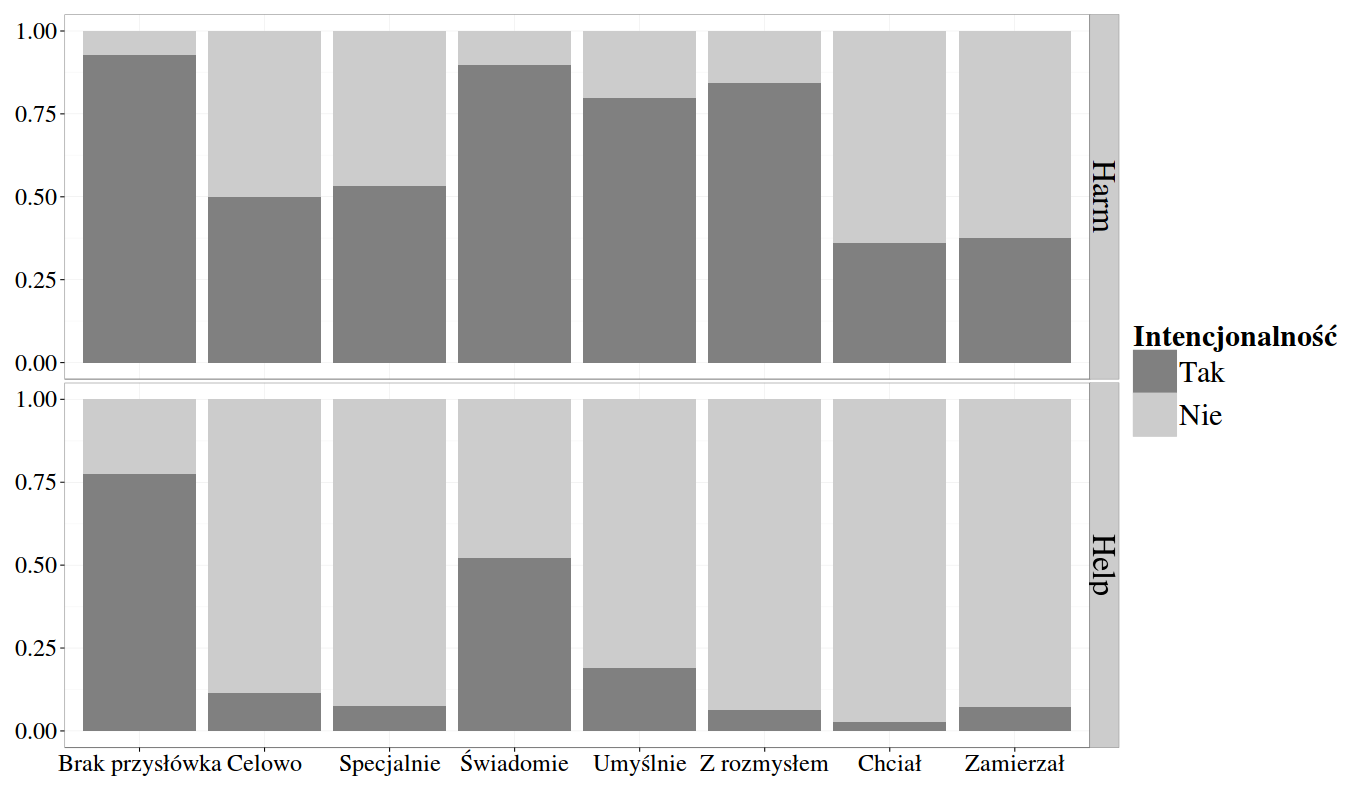
\includegraphics{bwp_chart1.png}
\end{figure}

 \section{Dyskusja}\label{sec:page-layout}
 \begin{fullwidth}
 \textsc{Analizy na gruncie programu pozytywnego} zakładają pewien uniwersalizm, przejawiający się w założeniu, że pojęcia intencji i intencjonalnego działania mają charakter fundamentalny i są niezależne od kultury. Być może jest to siatka pojęciowa właściwa tylko językowi angielskiemu. Dopiero badania w różnych społecznościach językowych mogłyby dać wgląd w to, co w tych pojęciach jest niezmienne i uniwersalne. Wówczas filozofia eksperymentalna mogłaby mieć wkład w rozumienie pojęć

 
 \noindent \textsc{W obrębie programu negatywnego} twierdzono, że uniwersalność efektu Knobe'a pokazuje nieadekwatność fotelowych analiz pojęciowych. Jego językowa interpretacja może posłużyć do podważenia tego argumentu. Jeżeli występowanie i rozmiar asymetrii zależy od użytych w eksperymencie wyrażeń wskazujących na intencjonalność działania, to efekt Knobe'a może być tylko artefaktem językowym. Wyniki wskazują, że odpowiedzi badanych w scenariuszach Knobe'owskich zależą nie tylko od ich pojęcia intencjonalnego działania, ale też od trudnych do wyodrębnienia czynników językowych.
 

\end{fullwidth}

\end{document}